

\begin{frame}{518 only}
    1 page - tie your research interests to the Astro2020 Decadal or the PlanetaryDecadal2022 surveys and list possible targets for an observing proposal that relates to priority science. 
    This does not need to be an original experiment, re-observing targets or reproducing past work that the Decadal rests on is \textit{preferred}.
    You are encouraged to reach out to scientists in Steward and LPL: \url{https://www.as.arizona.edu/people/faculty}, \url{https://www.lpl.arizona.edu/faculty}.
    You don't need to worry about the observatory capabilities, yet.
\end{frame}
\begin{frame}{Observing Proposal Prep}
    
The Steward Observatory 2.3 m ``Bok'' telescope is of Ritchey-Cretién design.% with a scale at the focal plane of 10”/mm. 
 Details: \url{https://lavinia.as.arizona.edu/~tscopewiki/doku.php?id=public:kitt_peak:bok_90:bok_90_telescope}
 
 \begin{enumerate}
 \item derive the thin lens equation
\item Calculate the f-number of secondary mirror when the telescope is f/9
\item Calculate the plate scale at prime focus
\item What is the distance from the primary to prime focus?
\item draw these configurations of the telescope with distances labelled
\end{enumerate}
\end{frame}

\begin{frame}{Point source part I)}
Williams et al 2004 describes the 90 prime instrument and Lesser and Vu 2004 describe the sensors:
\begin{enumerate}
    \item Find the typical read noise and gain
    \item Find the typical dark noise
    \item  estimate by eye the average QE in V-band
    \item estimate by eye the reflectivity of the aluminum primary mirror
    \item count the number of optics and calculate the system throughput, assume 2\% anti-reflection coating losses and an aluminum coated primary mirror
    \item Calculate the scattered light background per pixel and per 1 arcsec sq. PSF for a solar zodiacal background of 22 magnitudes/as$^2$ and no moonshine. 
    \item calculate the time to SNR for a seeing limited 15th magnitude point source, including the terms above
\end{enumerate}
    
\end{frame}

\begin{frame}{Point source part II)}

Identify a point source of interest and its key parameters, using Simbad (\url{simbad.cds.unistra.fr/simbad}) or JPL Ephemeris and any other resources necessary:

 \begin{enumerate}
\item describe the targets key parameters, including at least V-mag, RA, and DEC
\item Calculate the flux from the target in photons/cm$^2/\AA $/sec in the band of interest
 \item estimate the exposure time necessary to reach SNR=5 and SNR=100
 \item if this exposure time is impractical ($\gtrsim$2hrs), revisit your assumptions or target and repeat
 \item Why would you want to reach SNR 100 rather than 5?
 \item list any special considerations
\end{enumerate}
\end{frame}

\begin{frame}{Extended source}
Same as point source but for an extended source (solar system through extra-galactic is acceptable).

 \begin{enumerate}
 \item repeat point source but add surface brightness.
\end{enumerate}
\end{frame}





\begin{frame}{Source availability}

 \begin{enumerate}
 \item install astroplan: \url{https://github.com/astropy/astroplan}
 \item run the basic tutorials: \url{https://astroplan.readthedocs.io/en/latest/tutorials/summer_triangle.html}
 \item adjust the location to KPNO and your selected targets
 \item create an observing plan that allows you to get to your targets, based on the time to SNR from the previous problem
 \item make a plot that shows all your targets of interest in airmass vs local time
 \item form an ad-hoc telescope allocation committee with other students on your night(s) and generate an observing plan that allows everyone to observe, revising your targets and exposures times as necessary 
 \item  assume you might have to adapt the plan without internet:
 \begin{itemize}
    \item write the plan and key parameters in your notebook
     \item print out finder charts
 \end{itemize}
\end{enumerate}
\end{frame}

\begin{frame}{Code review}

you will be randomly assigned a classmates SNR code calculation code to review. 
Review the Google Code Review docs: \url{https://google.github.io/eng-practices/review/reviewer/looking-for.html}

Concentrate on:
 \begin{enumerate}
 \item does the code run?
 \item is it clear what each line does and why?
 \item does it follow the python style guide: \tiny{\url{https://peps.python.org/pep-0008/\#a-foolish-consistency-is-the-hobgoblin-of-little-minds}}
\end{enumerate}

\end{frame}


\begin{frame}{Observing Report - 518 only}
 \begin{enumerate}
 \item Use AASTex \url{https://journals.aas.org/aastexguide/} 
 \item motivate the measurement with an explicit citation to a decadal survey.
 \item substantiate or cite any assumptions
 \item present equations even if they appear trivial
\item Report measured read noise (electron/sec), bias (ADU), dark rate (electrons/sec), and gain (electrons/ADU).
\item Report measured count rate from your point source and extended source
\item Report SNR of both a point source and an extended source
\item report photometric brightness of your sources in Janskys and magnitudes (per sq arcsec for the extended source)
\item suggest future improvements and astrophysical significance in your conclusion
\end{enumerate}
\end{frame}


\section{HW2}

\begin{frame}{Echelle Spectroscopy}

 \begin{enumerate}
 \item Consider the design of a diffraction grating spectrometer for a 10 m telescope. The 2-pixel resolution
element is 0.5” and the required resolving power is R=20,000. Assume that the configuration is Littrow.
Two gratings are available, a first-order grating blazed at 17.5° and an echelle grating blazed at 63.5°.
Determine the collimator size required in both cases. Which is more practical?
\item Assuming the telescope
provides a F/15 beam, what is the focal length of these two collimators?
\end{enumerate}
\end{frame}


\begin{frame}{Basic Questions}
 \begin{enumerate}
 \item Derive the thin lens formula.
\end{enumerate}

\end{frame}


\begin{frame}{Spatial Frequencies}
The figure on the next page shows 1D cross sections of reflectivity and optical path error versus distance across the optic for an ideal D=8.4 m telescope primary mirror:

a)	Assume a 8.4 cm pitch lap runs is miscalibrated and adds a sinusiodal 100 nm RMS wavefront error at a spatial frequency equal to one over its size, and just along one axis. Draw new a new cross section of the OPD along the axis of the error and label the peak-to-valley error.
b)	Draw a two dimensional representation of the mirror with this error
c)	Calculate the Fourier series or estimate it by eye and draw the resultant 1D PSF cross section and sketch a 2D representation of this new PSF at 1 micron. Label both drawings in arcseconds and units of l/D. l is a wavelength of 1 micron.
d)	In signal processing the Nyquist frequency, one half the sampling rate of a system, is the minimum frequency that can be measured by the system. By this analogy, how many wavefront sensor elements and deformable mirror actuators would be required to correct this primary mirror error?
\end{frame}
\begin{frame}{Spatial Frequencies Figure}
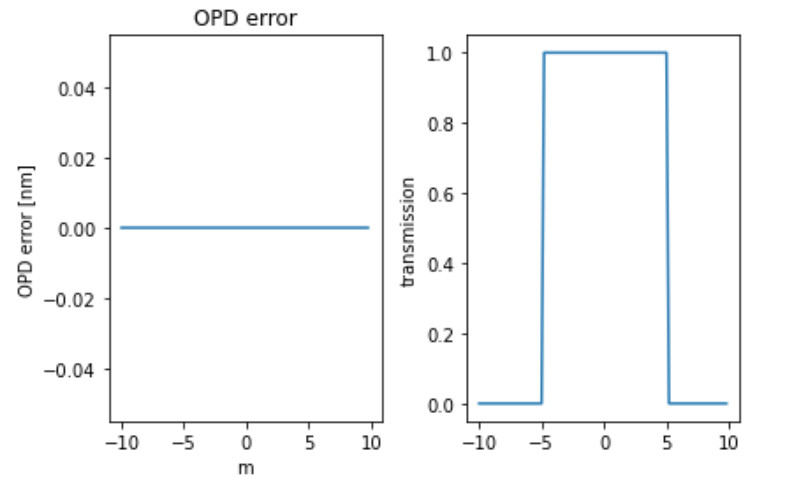
\includegraphics[width=0.9\textwidth]{figs/OPD_trans.png}
\end{frame}